% options:
% thesis=B bachelor's thesis
% thesis=M master's thesis
% czech thesis in Czech language
% slovak thesis in Slovak language
% english thesis in English language
% hidelinks remove colour boxes around hyperlinks

\documentclass[thesis=B,czech]{FITthesis}[2012/06/26]

\usepackage[utf8]{inputenc} % LaTeX source encoded as UTF-8

\usepackage{graphicx} %graphics files inclusion
% \usepackage{amsmath} %advanced maths
% \usepackage{amssymb} %additional math symbols

\usepackage{dirtree} %directory tree visualisation 
\RequirePackage{pdfpages}
\usepackage{float}
\usepackage[all]{nowidow}

% % list of acronyms
% \usepackage[acronym,nonumberlist,toc,numberedsection=autolabel]{glossaries}
% \iflanguage{czech}{\renewcommand*{\acronymname}{Seznam pou{\v z}it{\' y}ch zkratek}}{}
% \makeglossaries

\newcommand{\tg}{\mathop{\mathrm{tg}}} %cesky tangens
\newcommand{\cotg}{\mathop{\mathrm{cotg}}} %cesky cotangens

% % % % % % % % % % % % % % % % % % % % % % % % % % % % % % 
% ODTUD DAL VSE ZMENTE
% % % % % % % % % % % % % % % % % % % % % % % % % % % % % % 

\department{Katedra Softwarového inženýrství}
\title{Webový frontend informačního systému}
\authorGN{Jakub} %(křestní) jméno (jména) autora
\authorFN{Doležal} %příjmení autora
\authorWithDegrees{Jakub Doležal} %jméno autora včetně současných akademických titulů
\author{Jakub Doležal} %jméno autora bez akademických titulů
\supervisor{Ing. Jiří Chludil}
\acknowledgements{Chtěl bych poděkovat mojí rodině za podporu v době studií a při tvorbě této práce. Dále bych rád poděkoval mému vedoucímu Ing. Jiřímu Chludilovi za jeho příkladné přátelské vedení. A v neposlední řadě chci poděkovat Bc. Michaeli Voříškovi z firmy MAHALUX s.r.o. za jeho rady a vztřícnost.}
\abstractCS{Cílem této bakalářské práce je návrh, implementace a otestování webového frontendu informačního systému pro firmu MAHALUX s.r.o. Hlavním účelem aplikace je zefektivnění a centralizování evidence provozních dat firmy.
	
	Na základě sběru požadavků a analýzy firemních procesů je navržen informační systém s~webovým frontendem, který je implementovaný pomocí frameworku ReactJS v~jazyce JavaScript. Serverová část aplikace je realizována ve skriptovacím jazyce PHP s~využitím frameworku Nette. Aplikace byla podrobena uživatelskému testování použitelnosti.
	
	Výsledkem práce je informační systém spustilný v~běžném webovém prohlížeči. 
}
\abstractEN{The object of this bachelor thesis is to design, implement and test web frontend of information system for MAHALUX s.r.o. company. Application's main purpose is to make data storing more efficient and centralized.

Design of the web frontend is given by the system specification requirments from contracting company. It is implemented with usege of ReactJS framework in JavaScript language. Server-side application is made with PHP language and Nette framework. Usability testing was done on the application.

The outcome is the information system which you can run in every common web browser.
}
\placeForDeclarationOfAuthenticity{V~Praze}
\declarationOfAuthenticityOption{4} %volba Prohlášení (číslo 1-6)
\keywordsCS{webový frontend, informační systém, návrh, implementace, testování, hromadné zadávání dat, ReactJS, PHP, Nette framework}
\keywordsEN{web frontend, information system, design, implemtation, test, bulk data input, ReactJS, PHP, Nette framework}
% \website{http://site.example/thesis} %volitelná URL práce, objeví se v tiráži - úplně odstraňte, nemáte-li URL práce


\begin{document}

% \newacronym{CVUT}{{\v C}VUT}{{\v C}esk{\' e} vysok{\' e} u{\v c}en{\' i} technick{\' e} v Praze}
% \newacronym{FIT}{FIT}{Fakulta informa{\v c}n{\' i}ch technologi{\' i}}

\begin{introduction}
	MAHALUX s.r.o. je mladá expandující firma zabývající vývojem, výrobou a prodejem elektronických zařízení. Zároveň provozuje internetový obchod, kde nabízí vlastní produkty a distribuje zboží z~jiných eshopů. I~přesto, že firma existuje poměrně krátce, již expeduje po celém světě. To přináší velké nároky na evidenci rozličných dat o~adresách, bankovních spojeních a dalších informacích o~zákaznících. Proto se firma MAHALUX s.r.o. rozhodla pro zavedení informačního systému s~webovým frontendem, který přinese potřebné centralizované ukládání dat a pohodlný přístup k~těmto datům. Dalším hlavním účelem systému je zefektivnění procesu vyřizování objednávek.
	
	V~práci se zabývám analýzou, návrhem, implementací a testováním webového informačního systému.
	Úkolem úvodní části práce je sběr funkčních a nefunkčních požadavků zadavatele. Dále je také nutná analýza složitějších případů užití a firemních procesů. Následuje návrh struktury systému, komponentového prototypu a uživatelského rozhraní. Navazovat bude samotná implementace prototypu frontendu v~knihovně ReactJS a vytvoření serverové části aplikace v~jazyce PHP s~pomocí frameworku Nette. V~závěrečné kapitole je popsáno testování aplikace.
\end{introduction}

\chapter{Cíl práce}
	Cílem úvodní části práce je analýza požadavků zákazníka, prozkoumání složitějších případů užití a pochopení firemních procesů. Kromě toho je potřeba seznámení s~existujícími řešeními webových frontendů pro získání přehledu o~best practicies.
	
	Cílem praktické části práce je návrh, implementace a otestování webového frontendu tohoto informačního systému. Hlavní důraz bude kladen na dynamičnost uživatelského rozhraní. To by mělo uživateli napomáhat k~co nejrychlejšímu a bezchybnému vkládání dat. K~tomu budou využity šablony, které si uživatel nadefinuje společně s~daty a ty následně ze šablony vloží do konkrétního formuláře. Dále by měla být zajištěna přehledná reprezentace větších záznamů a hromadné úpravy. Systém bude komponentový pro zaručení možnosti jednoduchého rozšíření systému.
	
\chapter{Analýza}

\section{Specifikace systémových požadavků}

	Na základě diskuze s~firmou MAHALUX s.r.o. byly stanoveny následující systémové požadavky.
	
\subsection{Funkční požadavky}

\begin{enumerate}
	\item[FN1] Agenda faktur a fakturovaných katalogových položek(fakturováno může být několik katalogových položek v~počtu jeden a více).
	\begin{itemize}
		\item Přehled evidence vydaných faktur a fakturovaných položek a pro jednotlivé faktury:
		\begin{itemize}
			\item vytvoření nové faktury,
			\item editace faktury,
			\item smazání faktury a
			\item tisk faktury.
		\end{itemize}
		\item Formulář pro vytvoření a úpravu jedné nebo více faktur na základě jedné nebo více objednávek. Pro tento formulář zajistit předvyplnění fakturačních položek na základě položek v~objednávce či objednávkách.
		\item Přehled přijatých faktur a pro jednotlivé faktury:
		\begin{itemize}
			\item uložení přijaté faktury včetně souborů,
			\item změna stavu faktury (přijatá, částečně uhrazená, uhrazená),
			\item smazání faktury a
			\item tisk faktury.
		\end{itemize}
	\end{itemize}	
	\item[FN2] Evidence nabízených produktů a s~tím spojené
	 	vyhledání, přidání, úprava a smazání nabízeného produktu.
	\newpage
	\item[FN3] Agenda firemního skladu.
		\begin{itemize}
			\item Evidovat skladové pohyby u~jednotlivých produktů.
			\item Přehled položek ve skladu.
			\item Editace položek skladu.
		\end{itemize}
	\item[FN4] Agenda objednávek -- přehled evidovaných objednávek a pro jednotlivé objednávky:
	\begin{itemize}
		\item vložení nové objednávky,
		\item editace objednávky,
		\item smazání objednávky,
		\item vytvoření faktur na základě jedné nebo více objednávek a
		\item evidence trackingu po expedování.
	\end{itemize}
	\item[FN5] Formulář pro přípravu expedice položek objednávky.
	\begin{itemize}
		\item Formulář zobrazí objedané množství produktů a množství produktů na skladě. 
		\item Ve formuláři se přednastaví množství k~odeslání podle toho, zda je možné objednávku kompletně vybavit či ne. Pokud lze objednávky vybavit kompletně, nastavená hodnota bude rovna objednanému množství. Pokud nepůjde odbavit objednávku kompletní, bude nastavena hodnota 0.
		\item Expeditér bude dále moci upravit množství k~odeslání na hodnoty v~rozmezí 0 až objednané množství nebo množství na skladě podle toho, která hodnota je menší.
		\item Potvrzením vložení do expedice při nenulovém množství k~odeslání dojde k~vytvoření záznamu o~balíčku a jeho zařazení do následující expedice.
	\end{itemize}
	\item[FN6] Agenda dodávek.
	\begin{itemize}
		\item Přehled objednaných dodávek včetně trackingu.
		\item Formulář pro vložení nové dodávky včetně trackingu.
		\item Editace dodávky v~případě špatně nebo nekompletně dodané dodávky.
		\item Označení dodávky jako dodané způsobí automatické naskladnění.
	\end{itemize}
	\item[FN7] Agenda kontaktů.
	\begin{itemize}
		\item Na základě příznaku evidovat dodavatele a odběratele.
		\item Evidovaní budou dodavatelé -- právnické osoby.
		\item Evidence odběratelů:
		\begin{itemize}
			\item právnické osoby a
			\item fyzické osoby.
		\end{itemize}
		\item Evidovat kontakty tržních míst.
	\end{itemize}

	\item[FN8] Hromadné úpravy.
	\begin{itemize}
		\item Více záznamů lze editovat jako jeden. 
		\item Pokud jsou původní hodnoty stejné, zobrazí se k~úpravě stejně, jako by se editoval jeden záznam. 
		\item Pokud jsou původní hodnoty rozdílné, namísto pole k~editaci se zobrazí tlačítko pro výběr jedné společné hodnoty (ideálně histogram), kterou lze potom opět editovat jako jednu hodnotu. Pokud se hodnota neupraví, zůstávají původní hodnoty.
	\end{itemize}
	\item[FN9] Vyplnění formuláře šablonou.
	\begin{itemize}
		\item Uživatel si nadefinuje šablonu s~konkrétními daty v~konkrétních polích a šablonu uloží. 
		\item Při dalším vyplňování téhož formuláře bude moci vybrat uloženou šablonu a ta mu formulář vyplní uloženými daty. 
		\item Uživatel bude dále moci data upravit a případně šablonu upravit či uložit novou.
	\end{itemize}
	\item[FN10] Správa uživatelů.
	\begin{itemize}
		\item O~každém uživateli evidovat loginID, username, skutečné jméno, heslo.
		\item Každý uživatel má nějaké oprávnění. Oprávnění mohou být admin, expeditér.
		\item Založení uživatele.
		\item Upravení uživatele.
		\item Deaktivace uživatele.
		\item Přehled uživatelů.
		\item Administrátor bude moci vygenerovat uživateli nové heslo v~případě zapomenutí hesla.
	\end{itemize}
	\item[FN11] Evidence úprav dat (kdo data upravil a kdy).
	\begin{itemize}
		\item Pro každý záznam ve všech tabulkách bude evidováno kdo a kdy řádek vytvořil, upravil a smazal(technika soft delete).
		\item Informace o~tom, kým byla data upravena, bude zaznamenána z~loginu uživatele.	
	\end{itemize}
	\item[FN12] Vytvořit API pro manipulaci s~daty ve všech tabulkách.
\end{enumerate}

\subsection{Nefunkční požadavky}
\begin{enumerate}
	\item[NF1] Odezvy v~reálném čase (typicky maximálně 100 ms na 1000000 záznamů, u~větších tabulek základní stránkování s~použitím indexů).
	\item[NF2] Konzistence dat - na úrovni DB transakcí (server splňuje ACID).
	\item[NF3] Dynamicky reagující formuláře.
	\begin{itemize}
		\item Určená pole formuláře reagují na změnu v~jiném poli. Například při výběru/zadání hodnoty v~kolonce země se v~návaznosti na to upraví nabídka v~kolonce stát. 
		\item Pokud je pro dané pole možné vyplnit pouze jednu hodnotu, bude tato hodnota automaticky doplněna.
	\end{itemize}
	\item[NF4] Dynamické doplňování zapisovaného textu (našeptávač).
	\begin{itemize}
		\item Při zapisování údaje do určené kolonky systém automaticky napovídá zbylou část textu.
		\item Je potřeba, aby našeptávač mohl našeptávat z~více sloupců.
		\item Našeptávač se bude využívat při odkazování na informace z~jiné tabulky. Například při výběru položky z~objednávky, našeptávač našeptává počet kusů z~tabulky položky objednávky a název položky z~tabulky číselníku. Vždy budou určeny konkrétní sloupce z~odkazované tabulky.
	\end{itemize}
	\item[NF5] Tabulka pro zobrazení záznamů z~databázové tabulky.
	\begin{itemize}
		\item Editace řádků v~modálním okně. Zobrazení upravených dat až po odeslání na server a jejich opětovném načtení.
		\item Možnost zobrazit subtabulku pro jednotlivé řádky k~vypsání souvisejích položek.
		\item Globální filtrování záznamů v~tabulce nad všemi sloupci a textové filtrování nad všemi sloupci.
	\end{itemize}
\end{enumerate}

\subsection{Požadavky na rozhraní}
\begin{enumerate}
	\item[PR1] Integrace do MySQL databáze a souborového systému pro upload příloh.
	\item[PR2] Přívětivé uživatelské rozhraní v~ReactJS napomáhající uživateli práci odvést rychle a bezchybně.
\end{enumerate}

\section{Doménový model}
	Doménový model\ref{domain_model} popisuje entity a vazby mezi nimi v~doméně internetového obchodu firmy MAHALUX s.r.o. Hlavní pozornost je zaměřena na objednávky a infrastrukturu procesu jejich vyřizování. Objednávka má vždy seznam položek objednaných produktů a jejich množství. Množstvím se rozumí počet kusů nebo číselnou hodnotu nějaké veličiny, například délky či váhy. U~objednávky se dále evidují informace o~zákazníkovi v~závislosti na tom, zda jde o~fyzickou či právnickou osobu. O~fyzické osobě je zaznamenáno jméno a příjmení a o~právnické osobě pak název společnosti a daňové ID. Dále se eviduje doručovací adresa a také, pokud je odlišná od doručovací, fakturační adresa.
	
	V~návaznosti na objednávky vznikají balíčky s~objednanými produkty k~odeslání zákazníkovi. O~balíčcích jsou vedeny následující informace: hmotnost v~kilogramech, množství objednaného produktu v~balíčku, doručovací služba, která balíček doručuje, a pokud je k~dispozici, tak také internetová adresa pro sledování balíčku, neboli tracking. Dále platí, že objednávka může být rozdělena do více balíčků a to i v~rámci jednotlivé položky. Proto je nutné zaznamenávat množství konkrétního produktu v~balíčku. Balíčky jsou pravidelně expedovány každý pracovní den ve várce pro jednotlivou doručovací společnost. Aktuálně se jedná pouze o~Českou poštu, s.p. U~těchto expedičních várek je evidováno datum provedení expedice a informace o~tom, zda byla várka vyexpedována.
	
	V~případech, kdy není možné objednávku kompletně vyexpedovat ze zásob skladu, vznikají zásobovací dodávky. U~těchto dodávek je opět nutné evidovat seznam položek s~objednaným množstvím produktu, tak jak bylo definováno pro objednávky. Dále se zaznamenávají informace o~dodavateli, datum objednání dodávky, stav dodávky a případně internetová adresa sledování dodávky. Dodavatelé bývají využíváni opakovaně.
	
	Na základě přijatých zásobovacích dodávek(naskladnění) a vyexpedovaných objednávek(vyskladění) vznikají pohyby na skladě. Každý skladový pohyb je způsoben jednou z~těchto dvou událostí. Je nutné evidovat množství produktu, znamenající pohyb skladu, stejně jako u~položek objednávek a dodávek. Vyskladnění znamená skladový pohyb se záporným množstvím. Naskladnění je naopak pohyb s~kladným množstvím.
	
	Nezávisle na objednávkách je vedena evidence faktur, a to jak vydaných, tak i těch přijatých. Pro faktury vydané je znovu třeba ukládat seznam fakturovaných položek a jejich množství. Dále faktura obsahuje informace o~zákazníkovi. Opět se jedná o~různé údaje podle toho, zda se jde o~fyzickou či právnickou osobu. 
	
\begin{figure}
	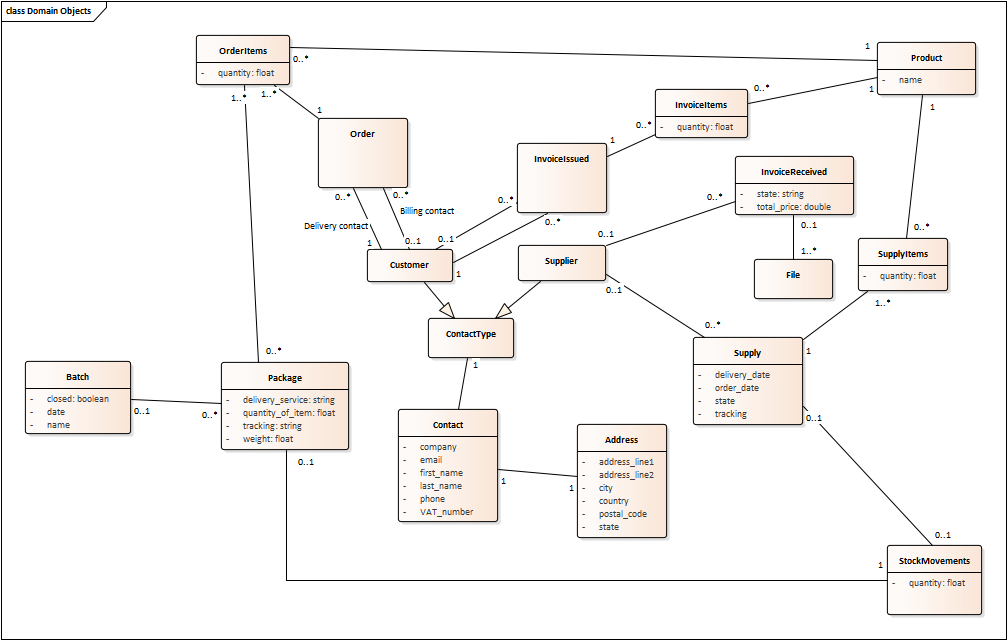
\includegraphics[height=\textwidth, angle=90]{domain_model.png}
	\caption{Doménový model}\label{domain_model}
\end{figure}

\section{Diagram procesu zpracování objednávky}
	Tento diagram \ref{order_activity} aktivit popisuje proces zpracování objednávky od jejího přijetí až po její vyřízení. Objednávku vytváří zákazník a dále ji odesílá firmě MAHALUX. Ta ji po přijetí zpracovává. Kontroluje se především, zda jsou odjednané produkty na skladě. V~závislosti na tom pak vznikají dodávky. Po kompletaci objednávky následuje její expedice. Ta může nastat i v~případě objednávky, která není kompletně na skladě, ale zákazník si ji přeje odeslat nekompletní. Po vyexpedování je zákazník informován o~předání zásilky dopravci.

\begin{figure}
	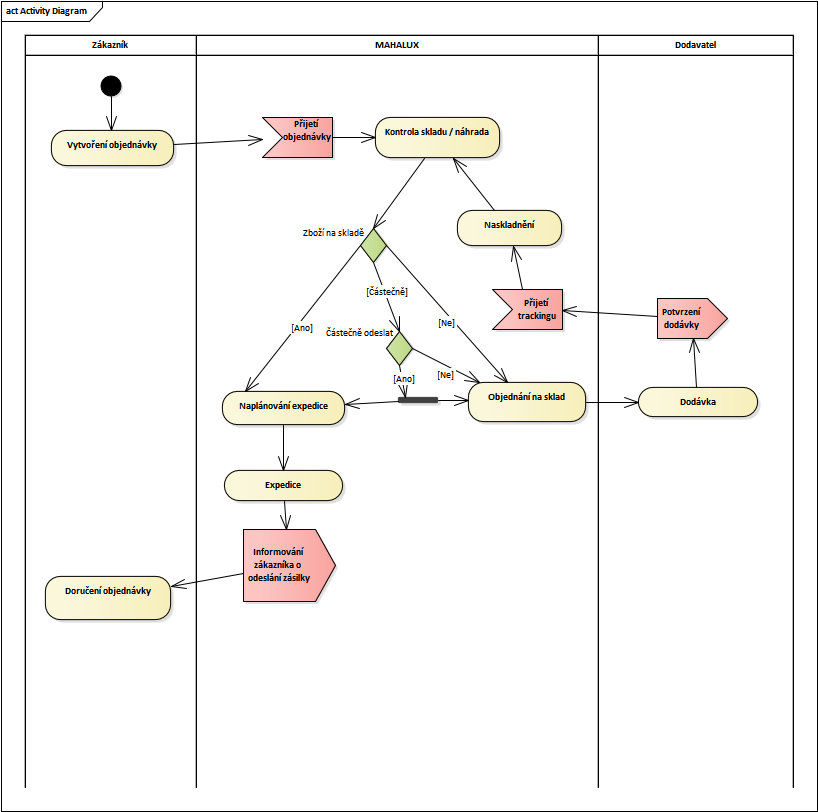
\includegraphics[width=\textwidth]{order_activity.png}
	\caption{Diagram procesu zpracování objednávky}\label{order_activity}
\end{figure}

\section{Životní cyklus objednávky}
	Na obrázku \ref{oredr_cycle} je znázorněn životní cyklus objednávky. Zajímavostí je například to, že pokud si zákazník přeje objednávku odeslat, i když není kompletně na skladu, objednávka se dostane do stavu \uv{Částečně v~expedici}. 
	
\begin{figure}
	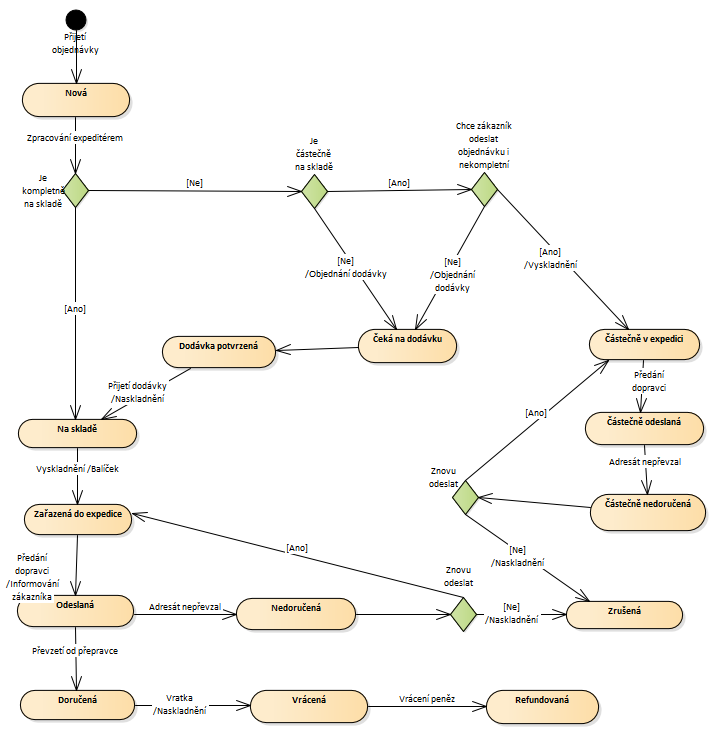
\includegraphics[width=\textwidth]{order_cycle.png}
	\caption{Životní cyklus objednávky}\label{oredr_cycle}
\end{figure}


\section{Použité technologie}

\subsection{ReactJS}
	ReactJS\cite{reactjs} je JavaScriptová knihovna zaměřená na vykreslování webových aplikací. Je založená na vizuálních komponentách, které při změně stavu aplikace efektivně překresluje. Tento proces je implementován pomocí virtualizace DOM, kterým je zaznamenáván stav skučného DOM. Při změně stavu je virtuální DOM porovnán se skutečným a následně je překreslena pouze dotčená část skutečného vzhledu stránky. \cite{react-crud-app}

	React je příkladem tzv. jednosměrného vázání dat. To znamená, že události uživatelského rozhraní jsou přenášeny do stavu aplikace   změnou modelu, která je provedena voláním metody \verb|setState|. Jde o~tzv. manuální detekci změny. React je tím informován o~modifikaci modelu a provede již zmíněný proces propagace změn do DOM.\cite{data_binding} Tento proces je znázorněn na obrázku \ref{data_binding}.

	\begin{figure}
		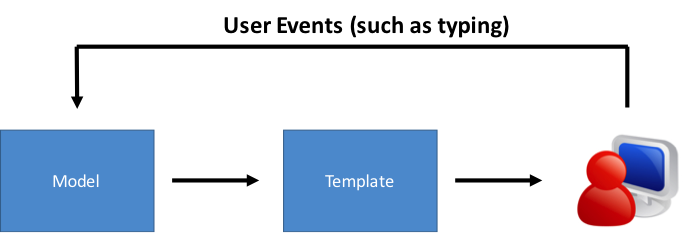
\includegraphics[width=\textwidth]{databinding2.png}
		\caption{Jednosměrné datové vázání}\label{data_binding}
	\end{figure}

	Pro definici toho, jak se má jednotlivá komponenta vykreslit, využívá React speciální jazyk JSX. Jde o~syntaktické rozšíření jazyku JavaScript, v~kterém je možné zapisovat HTML tagy. Může připomínat šablonovací systém, ale v~JSX lze zapisovat přímo příkazy JavaSciptu, jejich vložením do složených závorek. Díky JSX lze zapisovat kód pro vykreslování a ostatní logiku uživatelského rozhraní společně a získat tak lepší přehled o~aplikaci.\cite{jsx} 
	
\subsection{Nette Framework}
	Nette je kompletní framework pro PHP, který výrazně zjednodušuje tvorbu webových aplikací. Jeho autorem je český vývojář David Grudl. Je založen na samostatných knihovnách, které dohromady tvoří celý framework. Jednou z~hlavních předností Nette je vysoká míra zabezpečení za pomoci technologií, které eliminují všechny bezpečnostní mezery. Nette staví na architektuře MVC.\cite{nette}
	
	Model-View-Controller je softwarová architektura, která vznikla z~potřeby oddělit u~aplikací s~grafickým rozhraním kód obsluhy (controller) od kódu aplikační logiky (model) a od kódu zobrazujícího data (view). Tím jednak aplikaci zpřehledňuje, ale také usnadňuje budoucí vývoj a umožňuje testování jednotlivých části zvlášť.
	
	\begin{description}
		\item[Model] je datový a zejména funkční základ celé aplikace. Je v~něm obsažena aplikační logika. Jakákoliv akce uživatele (přihlášení, vložení zboží do košíku, změna hodnoty v~databázi) představuje akci modelu. Model si spravuje svůj vnitřní stav a ven nabízí pevně dané rozhraní. Voláním funkcí tohoto rozhraní můžeme zjišťovat či měnit jeho stav. Model o~existenci view nebo kontroleru neví.
		\item[View]-- neboli pohled, je vrstva aplikace, která má na starost zobrazení výsledku požadavku. Obvykle používá šablonovací systém a ví, jak se má zobrazit ta která komponenta nebo výsledek získaný z~modelu.
		\item[Controller]je řadič, který zpracovává požadavky uživatele a na jejich základě pak volá patřičnou aplikační logiku (tj. model). Poté požádá view o~vykreslení dat. Obdobou kontrolerů v~Nette Framework jsou presentery.\cite{nette_mvc}
	\end{description}

	Komunikace mezi jednotlivými částmi je znázorněna na obrázku \ref{mvc_arch}.

	\begin{figure}
		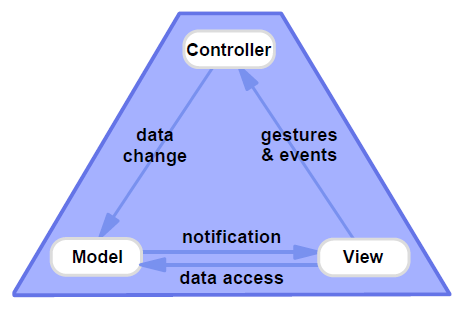
\includegraphics[width=\textwidth]{mvc.png}
		\caption{Architektura MVC}\label{mvc_arch}
	\end{figure}
	
\subsection{Doctrine 2}
	Doctrine 2 je ORM knihovna pro jazyk PHP. Zajišťuje mapování relační databáze na PHP objekty. Takové objekty se nazývají \uv{Entity}. Doctrine 2 je postavena na návrhovém vzoru Data Mapper reprezentovaném vůči zbytku aplikace fasádou v~podobě Entity Manageru. Pro definici vlastností jednotlivých entit se elegantně využívají komentářové anotace. Není tedy nutné entity dědit od nějakého společného předka a můžeme si hierarchii dědičností udělat zcela dle svých potřeb. Struktura databáze i veškeré její změny se generují automaticky z~definic entit pomocí nástroje schema-tool. \cite{doctrine2} 
	
	Schema-tool je nástroj pro manipulaci s~databázovým modelem používaný z~příkazové řádky. Na základě ORM anotací vytvoří databázové DDL skripty pro zavedení databázového schématu, které mohou být dále odladěny nebo automaticky provedeny.
	
	Doctrine 2 je rozdělena do tří vrstev:
	\begin{description}
		\item[Common] Definuje základní obecná rozhraní, třídy a knihovny. Například nástroje pro práci s~kolekcemi, anotacemi, cachováním, událostmi apod. Ty jsou pak využívány oběma vyššími vrstvami. Common sám o~sobě je ale na zbylých vrstvách nezávislý, takže je ho teoreticky možné používat i samostatně. Všechno, co sem patří, je definováno v~namespace \verb|Doctrine\Common|.
		\item[DBAL (DataBase Abstraction Layer)] Abstrahuje zbytek aplikace od konkrétního typu databáze. Primárně rozšiřuje standardní PDO, ale umí pracovat i s~jinými databázovými drivery. DBAL je závislý na Common, ale může být opět teoreticky používán i samostatně bez poslední ORM vrstvy. Vše, co je jeho součástí, se nachází v~namespace \verb|Doctrine\DBAL|.
		\item[ORM (Object-Relational Mapping)] je nejvyšší vrstva, která zajišťuje mapování aplikačních objektů na relační databázi, jejich persistování a načítání. ORM je závislá na DBAL i Common. Namespace této vrstvy je \verb|Doctrine\ORM|.\cite{doctrine2}
	\end{description}

\section{Výběr nástroje pro modelování tříd}
	Hlavním cílem bylo najít nástroj, který by uměl z~namodelovaného schématu vygenerovat třídní model včetně ORM notací pro Doctrine 2 a metod get a set. Takový nástroj by velice pomohl při vývoji. V~první řadě je potřeba pro vizualizaci problémové domény. Za druhé poskytne zdrojový kód modelu zastřešující databázové schéma. Vybíral jsem z~následujících dvou nástrojů.

\begin{description}
	\item[Enterprise Architect]
	je poměrně robustní UML nástroj pro modelování celého vývojového cyklu softwaru. Pokrývá vše od sběru požadavků, modelování business procesů, architektury, domény až po class diagramy, či databázové modely. Dále umožňuje generování zdrojových kódů modelu včetně getterů a setterů pro jazyky Java, C++, C\#, Python, PHP, aj., které provádí na základě modifikovatelných šablon.
	
	Tyto šablony využívají vlastní jazyk nazýváný Transformation Template language. Enterprise Architect také podporuje generování DDL skriptů pro mnoho databázových enginů jako jsou Oracle, MySql, SQL Server a další.\cite{enterprise_architect}

	\item[Skipper\cite{skipper}]
	je nástroj pro modelování E-R schémat zaměřený na programovací jazyk PHP. Umožňuje generovat zdrojový kód modelu s~ohledem na použitý MVC framework a také dle zvolené ORM knihovny. Tím například u~Doctrine 2 nepřímo zajistí i databázové schéma. To je vygenerováno pomocí schema-tool. Skipper podporuje ORM knihovny Doctrine, Doctrine 2, Propel a CakePHP.\cite{skipper_features}
\end{description}

	Skipper je bezesporu lépe připravený na ORM. Generování notace pro Doctrine 2 zvládá bezchybně. Enterprise Architect ORM neřeší. Na druhou stranu lze v~Enterprise Architectu generování kódu doupravit pomocí šablon a plně nakonfigurovat. To může být velmi užitečné, například při použití traitu společného pro všechny třídy reprezentující databázové entity. Programový kód pro použití traitu se jednoduše vloží do šablony. Skipper toto neumožňuje a přidání je nutné dělat ručně. Nicméně vyladění šablon v~nástroji Entreprise Architect pro generování zdrojového kódu včetně notace pro Doctrine 2 by bylo poměrně obtížné a s~nejistým výsledkem. Proto jsem se rozhodl pro využití Skipperu i přes jeho slabší konfigurovatelnost.	


\chapter{Návrh}

\section{Architektura}
Pro architekturu systému bude využita struktura Nette. Půjde tedy o~architekturu MVC(v případě Nette pojmenovanou MVP). Část uživatelského rozhraní bude generována pomocí Latte šablon. Zbytek webového frontendu bude sestaven z~vytvořených komponent React. Nette presentery budou taktéž využity pro vytvoření API.

\section{Model tříd}
	Návrhový model tříd si klade za cíl správně přiřadit zodpovědnost třídám. Dále také může popisovat použité návrhové vzory a programovací techniky.\cite{si1_pred6} Pro účely navrhovaného systému jsem model tříd rozdělil do dvou částí. V~první části, popisující reactové komponenty na klientské straně aplikace, jde spíše o~popis prototypů JavaScriptových objektů. V~drůhé části jsou poté vyobrazeny třídy pro jazyk PHP.
	
\subsection{Klientská strana}
	Komponenty Reactu jsou vytvářeny děděním od třídy React.Component, to lze pozorovat na obrázku \ref{ui_komponents}. Skládáním komponent jsou vytvářeny jednotlivé webové stránky.
	
\begin{figure}
	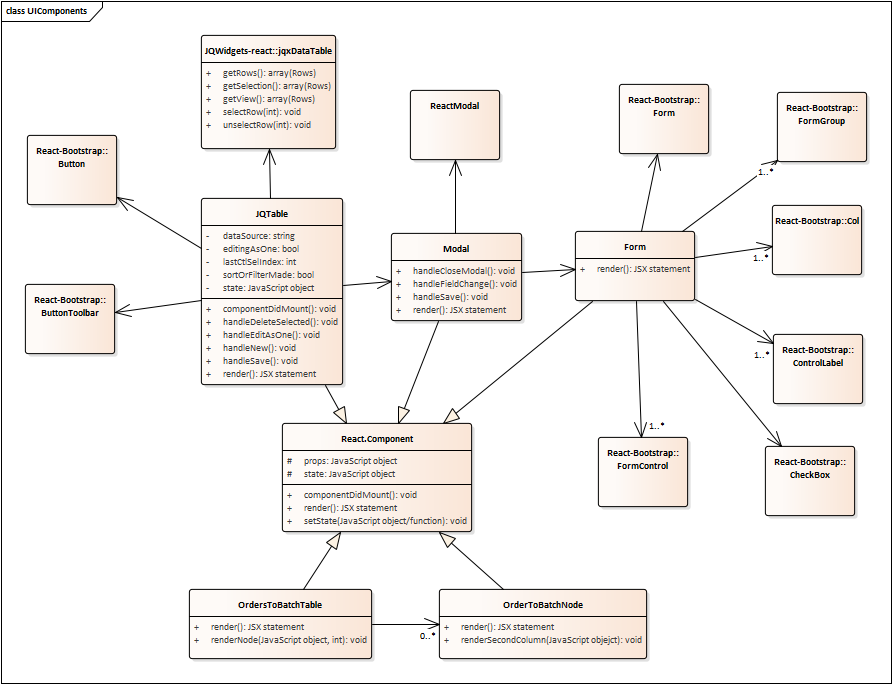
\includegraphics[width=\textwidth]{UI_components.png}
	\caption{Komponenty uživatelského rozhraní}\label{ui_komponents}
\end{figure}

\subsection{Serverová strana}
	Na serverové straně jsou využity knihovny frameworku Nette, a to především presentery a formuláře. Od samotné aplikace je pak oddělen modul API. Vše je znázorněno na obrázku \ref{server_side}.
	
\begin{figure}
	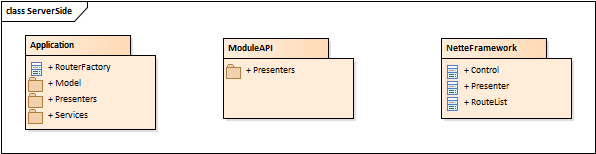
\includegraphics[width=\textwidth]{server_side.png}
	\caption{Balíčky serverové strany}\label{server_side}
\end{figure}

	Z~aplikace je nejzajímavější struktura presenterů, která je vyobrazena na snímku \ref{server_side_presenters}. Lze zde pozorovat architekturu MVP, kde model zastupují třídy *Service, view reprezentují šablony Latté a presentery představují samotné třídy *Presenter, které jsou odděděny od Nette Preseneteru.

\begin{figure}
	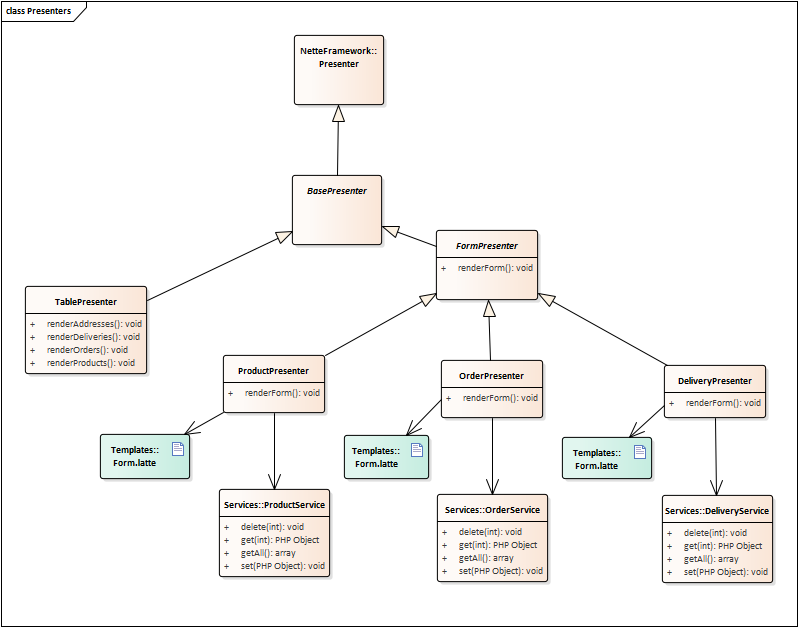
\includegraphics[width=\textwidth]{server_side_presenters.png}
	\caption{Presentery aplikace}\label{server_side_presenters}
\end{figure}	
	
	Podobně vypadá model presenterů API. Ačkoli zde ze zjevného důvodu chybí šablony pro vykreslování. Struktura prezenterů API je zachycena na diagramu \ref{api_presenters}.
\begin{figure}
	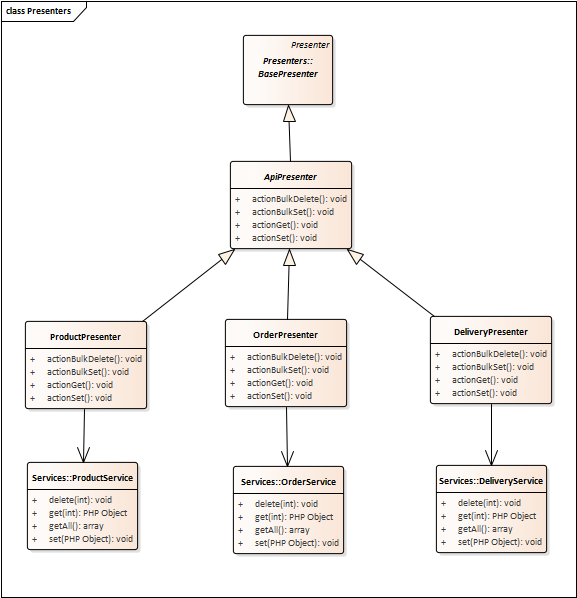
\includegraphics[width=\textwidth]{api_presenters.png}
	\caption{Presentery API}\label{api_presenters}
\end{figure}
	Dostupnost API je navržena přes URL <adresa-systému>/api.

\section{E-R model}
	E-R model\ref{er_model} popisuje relační databázový model, navržený pro vyvíjený systém. Model popisuje entity se všemi vlastnostmi a vazby mezi nimi. Je vytvořen v~programu Skipper, který vygeneruje zdrojový kód zastřešujících PHP datových objektů včetně notací pro ORM knihovnu Doctrine 2. Pomocí schema-tool je ze vzniklých tříd zavedeno databázové schéma. Vzhledem k~jeho rozsáhlosti byl model rozdělen do několika částí.
	
	První, tmavěji zelená sekce, popisuje evidované informace o~uživateli systému. Každý uživatel(User) může mít více rolí(UserRole) a zároveň každou roli může zaujímat více uživatelů. Jde tedy o~vazbu m:n. Tu realizuje vazební tabulka UserRoleUser. Vzhledem k~tomu, že každou roli může mít každý uživatel pouze jednou, tvoří primární klíč této tabulky dvojice cizích klíčů z~tabulek User a UserRole.
	
	Světle fialová oblast nastiňuje strukturu informací o~kontaktních adresách. Rozlišují se kontakty zákazníků, zaměstnanců firmy, firemní kontakty, kontakty dodavatelů a tržních míst. Všechny společné informace jsou vedeny ve společné tabulce Address. Typ kontaktu je rozlišen sloupcem diskriminátoru addressType. Všechny typy kontaktů dále mají, vlastní tabulky s~jejich specifickými informacemi. Tyto tabulky jsou vázány ke společné tabulce vazbou 1:1. Tato vazba je zajištěna cizími klíči v~tabulkách potomků, které jsou zároveň i klíči primárními. Dále je zaveden rejstřík zemí včetně jejich států(krajů). Země typicky mají několik států a stát náleží pouze jedné zemi. O~zemích je dále vedeno to, na kterém kontinentě se nacházejí.
	
	Tabulky popisují strukturu informací o~fakturách jsou v~bílé části, nacházející se vlevo dole. Evidence přijatých a vydaných faktur je vzájemně oddělena. U~vydaných faktur je důležité ukládat jednotlivé fakturované položky produktů a jejich množství. Fakturováno může být několik položek. Dále je pro každou vydanou fakturu nutné evidovat fakturační adresu zákazníka. K~přijatým fakturám jsou uloženy soubory reprezentující tyto faktury. Platí, že každý takový soubor může být pouze u~jedné evidované faktury. Dále je zaznamenána fakturovaná částka a stav zaplacení faktury. 
	
	Pro popis dodávek je použito žluté pole. U~dodávek je opět evidováno, jaké produkty obsahuje a v~jakém množství. K~dodávkám je pomocí cizího klíče uveden dodavatel, přepravní služba a volitelně i uživatel, který dodávku vytvořil. Přijetím dodávky vždy vzniká skladový pohyb s~kladným množstvím.
	
	V~tmavě růžové sekci je popsán sklad. Pro jednotlivé sklady je pomocí cizího klíče z~tabulky AddressOur evidováno to, na které adrese se sklad nachází. Pro každý sklad jsou dále evidovány skladové pohyby. Ty bývají inicovány již zmíněnými dodávkami nebo expedováním balíčku. Jedná se o~dva výlučné stavy. Nemůže nastat stav, že by skladový pohyb odkazoval na přijatou dodávku a zároveň na expedovaný balíček. Toto bude ošetřeno databázovým omezením Constraint, který toto bude kontrolovat.
	
	Expedované balíčky jsou znázorněny ve světle zeleném obdélníku. Balíček bývá zařazen do konkrétní expediční várky. V~této várce bývá více balíčků. U~balíčků je také nutné evidovat jejich soubory, typicky to jsou jejich fotografie. Podobně je tomu tak i u~kompletních várek. U~balíčku je také nutné znát doručovací službu. Tato služba bývá použita vícekrát. Zmiňované soubory jsou popsány v~bílé sekci. Soubory budou uloženy v~jejich binární podobě. U~fotografií bude vytvořen a uložen datově menší náhled fotografie. Pro textové dokumenty bude volitelně uložen jejich text získaný optickým čtením.

	Struktura schématu pro objednávky je zobrazena ve světle růžovém poli. Pro každou objednávku jsou evidovány jedntlivé řádky objednávky. Dále platí, že na každém řádku objednávky může být několik produktů v~libovolném množství. U~objednávky je dále nutné zaznamenat odesílací a fakturační adresu zákazníka. Volitelně pak adresu tržního místa a vlastní firemní adresu.
	
	V~tmavě modré oblasti je popsán model informací o~nabízených produktech. O~produktech jsou například evidovány jednotlivé jeho atributy. Každý definovaný atribut může být použit pro více produktů. U~produktů je také rozlišován jejich typ. U~typů produktů je určeno, zda jde o~fyzický produkt, službu, interní produkt nebo kombinace předchozích.
	
	Pro indexaci, a s~tím spojené rychlejší vyhledávání podle hodnot sloupců, jsem zvolil následující sloupce: 
	\begin{itemize}
		\item name z~tabulky Product,
		\item ourOrderUID z~tablky Order,
		\item lastName a email z~tabluky Address,
		\item name z~tabulky State,
		\item name z~tabulky Country a
		\item alias z~tabulky User.
	\end{itemize}
	Pro všechny vazby ve schématu je voleno výchozí nastavení pro operace delete a update a to akce restrict, která nepovoluje operace update a delete pro záznamy v~rodičovské tabulce mající potomky v~podřízené tabulce.
	
\begin{figure}
	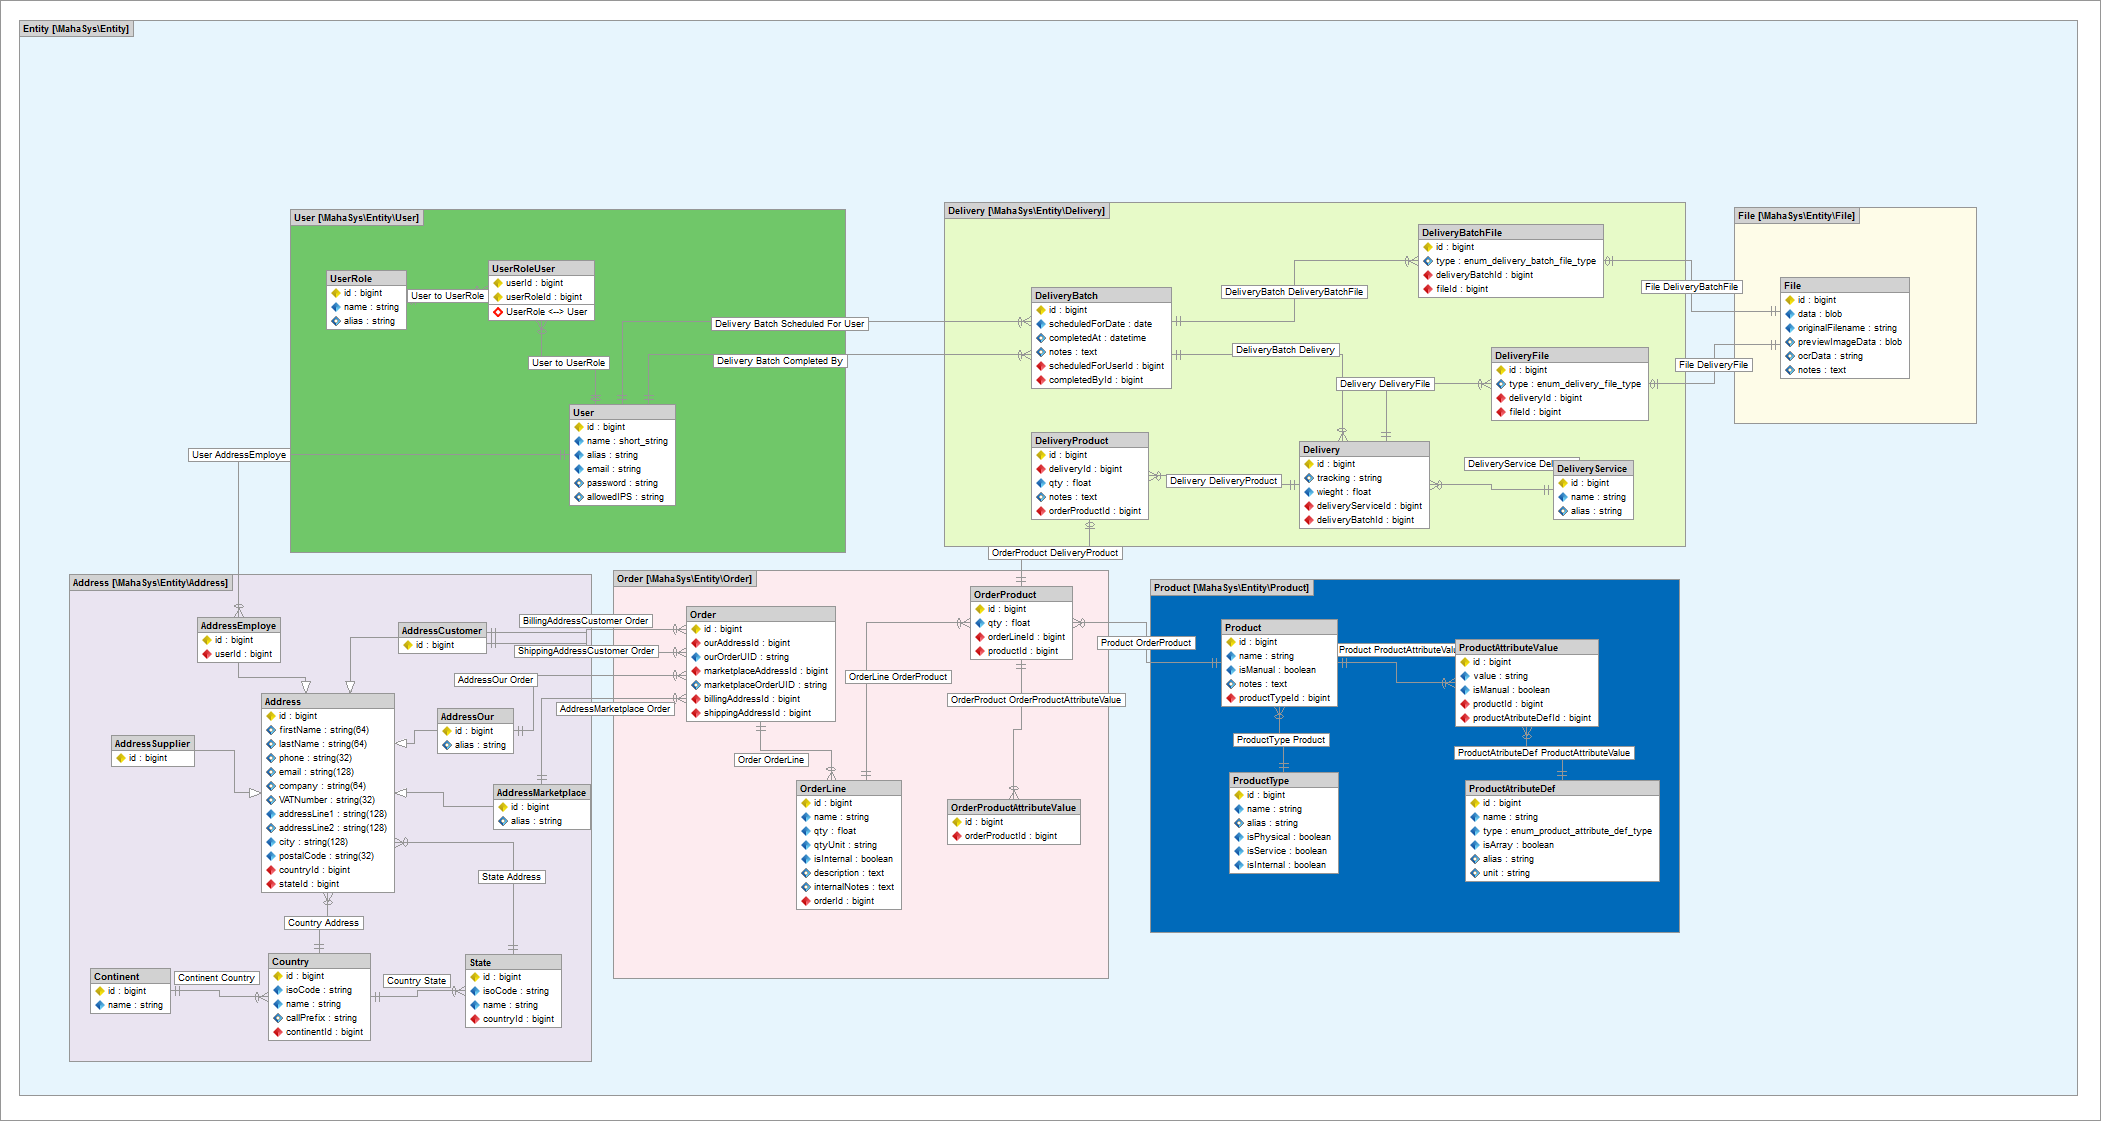
\includegraphics[width=500pt, height=\textwidth, angle=90]{mahasys_ermodel.png}
	\caption{E-R model}\label{er_model}
\end{figure}



\section{Uživatelské rozhraní}

\subsection{Formulář pro naplánování expedice}
	Na obrázku \ref{expedice} je navržený formulář pro naplánování expedice definovaný ve funkčním požadavku FN5. Jednotlivé ~řádky tabulky tvoří konkrétní objednávky. Řádky jsou dále rozděleny dle jednotlivých produktů v~objednávce. Textová pole s~plným okrajem a bílým tělem naznačují upravitelné atributy. Pole s~uživatelsky neupravitelným obsahem pak představují obdélníky se světle růžovým tělem a čárkovaným okrajem. V~jednotlivých sloupcích jsou zleva informace o~množství objednaného produktu, množství produktu které zbývá odeslat, množství ke vložení do balíčku, množství produktu na skladě, poznámka a váha zadaného množství produktu. V~posledním sloupci se pak nachází pole pro výběr doručovací služby a tlačítko \textbf{Schedule dispatch}, pomocí kterého dojde k~vytvoření balíčku se zadaným množstvím produktů v~systému. Tlačítko \textbf{Bulk: Schedule dispatch} poté simuluje stisknutí všech tlačítek \textbf{Schedule dispatch}.

\begin{figure}
	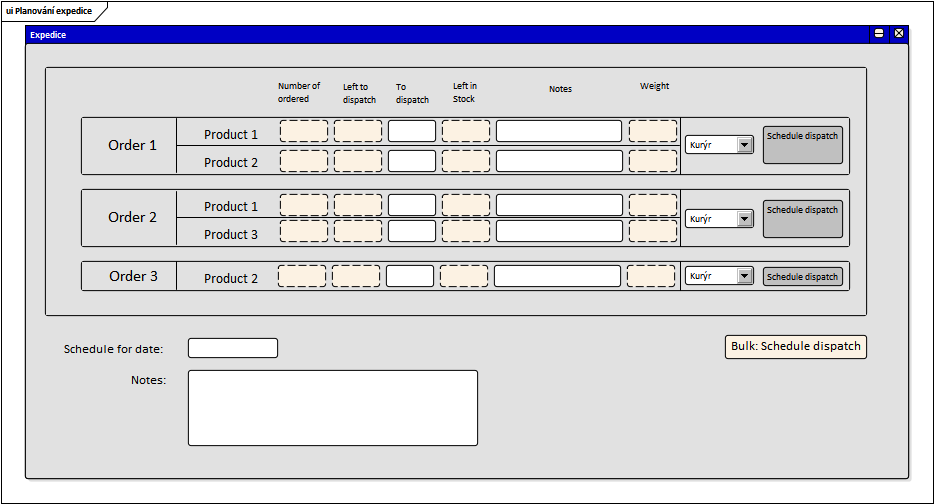
\includegraphics[width=\textwidth]{expedition_plan.png}
	\caption{Formulář pro naplánování expedice}\label{expedice}
\end{figure}

\subsection{Formulář pro vytvoření faktury}
	Formulář pro vytvoření faktury definovaný ve funkčním požadavku FN1 je nastíněn na obrázku \ref{faktura}. V~levé části se nachází seznam objednávek včetně objednaných položek. Položky půjde nezávisle na objednávce vkládat do fakturačních položek pomocí tlačítka \textbf{Billing}. Finální podoba fakturovaných položek bude zobrazena v~tabulce v~pravé dolní části formuláře. Fakturované množství produktů půjde upravit ve sloupci \uv{Qty} nebo položky z~faktury kompletně odstranit červeným tlačítkem \textbf{X}. Informace o~zákazníkovi budou vyplněny dle první vybrané objednávky nebo půjde zákazníka dohledat přes textové pole s~dymickým doplněním textu.

\begin{figure}
	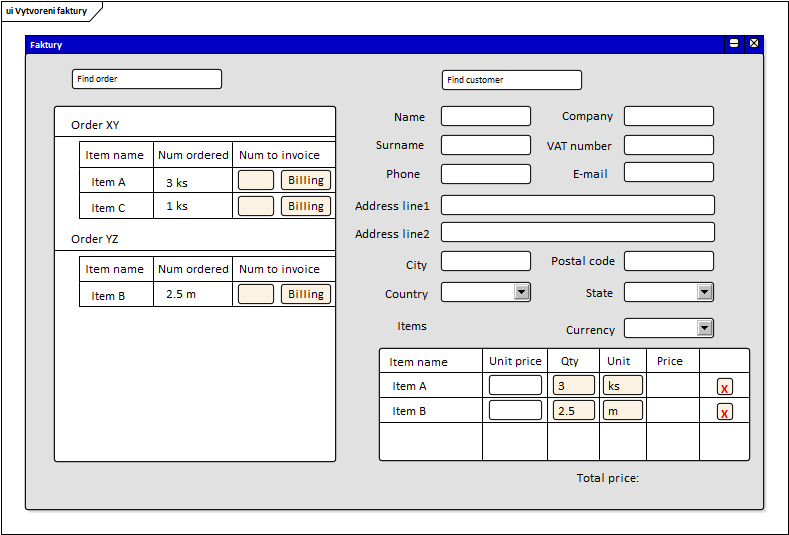
\includegraphics[width=\textwidth]{invoice_form.png}
	\caption{Formulář pro vytvoření faktury}\label{faktura}
\end{figure}

\subsection{Tabulka}
	Obrázek \ref{tabulka} zobrazuje navrženou tabulku pro zobrazení hodnot z~databáze. Základem tabulky je jqxDataTable\cite{jqx_dataTable} od jQWidgets. JqxDataTable poskytuje již hotové stránkování, textové řazení podle jednotlivých sloupců, textové pole pro filtrování a možnost zobrazit vloženou tabulku. Díky rozsáhlému API umožňuje vytvoření vlastního způsobu vybírání řádek. Komponenty od jQWidgets mají mnoho vlastních stylů. V~návrhové ukázce je použit styl \uv{Light}.
	
	K~prvkům jqxDataTable jsou doplněna tlačítka pro přidání nového záznamu, smazání záznamu nebo záznamů na základě výběru řádků a tlačítko pro hromadnou editaci řádků.

\begin{figure}
	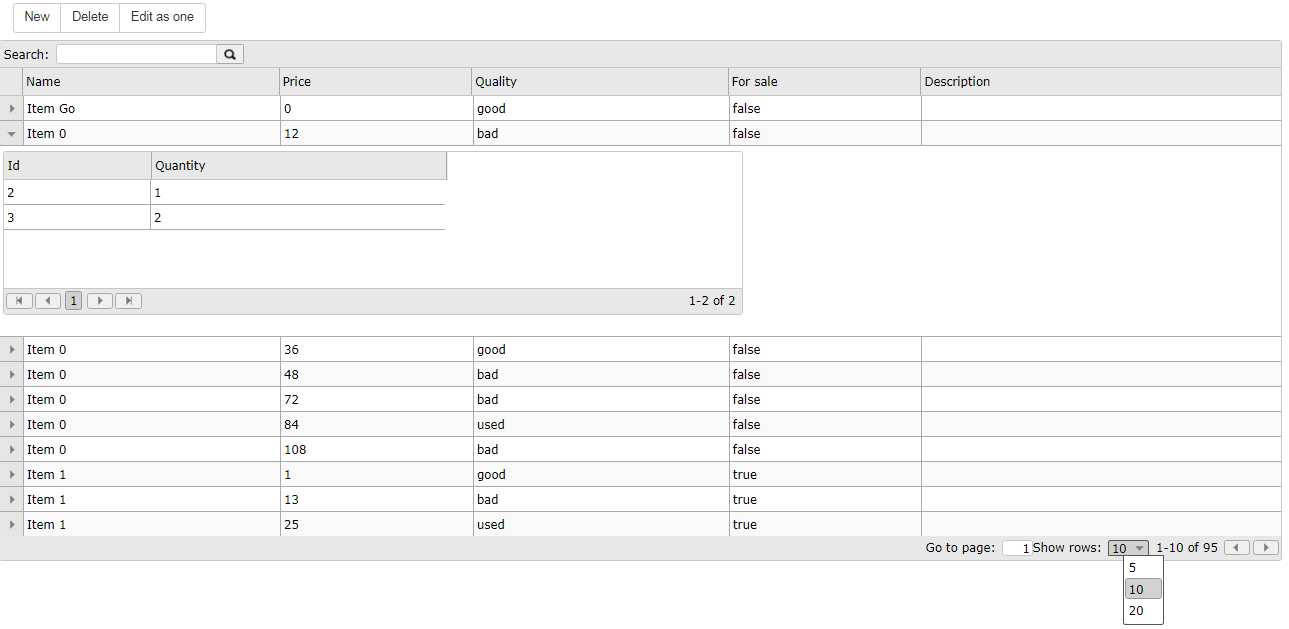
\includegraphics[width=500pt, height=0.8\textwidth, angle=90]{data_table.png}
	\caption{Tabulka}\label{tabulka}
\end{figure}
	

\chapter{Realizace}

\section{Instalační příručka}
	V~této kapitole je popsána instalace aplikace na Linuxové distribuci Debian~9.
\subsection{Instalace systému}
	Jako první provedeme instalaci Debianu 9 na náš stroj. Instalační obrazy jsou dostupné na stránce \url{https://www.debian.org/distrib/}. Obraz Debianu zahrnuje i webový server Apache2, jeho instalaci zajistíme zaškrtnutím volby \uv{web server} u~výběru komponent systému. Při zavádění systému taktéž vytvoříme uživatele \uv{mahasys}.
\subsection{Nastavení uživatele}
	Po instalaci systému bude dalším krokem nastavení vytvořeného uživatele. Nejprve za pomoci uživatele \uv{root} doinstalujeme nástroj sudo, a to příkazem \verb|apt-get intsall sudo|. Dále přidáme uživatele mahasys do skupiny uživatelů sudo pokynem \verb|adduser mahasys sudo|. Poté se pomocí \verb|su mahasys| přepneme na uživatele mahasys.
\subsection{Instalace PHP}
	Aplikace používá skriptovací jazyk PHP verze 7.2. Spuštěním následujících příkazů nainstalujeme tuto verzi PHP a její rozšíření.
	\begin{verbatim}
	sudo apt-get install apt-transport-https ca-certificates
	sudo wget https://packages.sury.org/php/apt.gpg
	sudo mv apt.gpg /etc/apt/trusted.gpg.d/php.gpg 
	echo "deb https://packages.sury.org/php/ stretch main" | 
	sudo tee /etc/apt/sources.list.d/php.list
	sudo apt-get update
	sudo apt-get install php7.2-cli libapache2-mod-php7.2
	sudo apt-get install php7.2-sqlite3 php7.2-mysql
	\end{verbatim}
\subsection{Nastavení PHP a Apache}
	Rozšíření naistalovaná v~předchozím kroku musíme povolit. Docíleme toho následujícími příkazy:
	\begin{verbatim}
		sudo phpenmod pdo_mysql
		sudo phpenmod pdo_sqlite
		sudo phpenmod sqlite3
	\end{verbatim}
	Nyní v~souboru /etc/apache2/apache2.conf upravíme nastavení složky\newline/var/www/ do nasledujícího tvaru.
	\begin{verbatim}
		<Directory "/var/www/">
		Options Indexes FollowSymLinks
		AllowOverride All
		Require all granted
		</Directory>
	\end{verbatim}
	Dále povolíme modul rewrite příkazem \verb|sudo a2enmod rewrite| a restartujeme Apache: \verb|sudo apache2ctl -k restart|.
\subsection{Stažení aplikace}
	Aplikaci nainstalujeme do složky /var/www/html. Přesuneme se do ní příkazem \verb|cd /var/www/html|. Samotnou aplikaci stáhneme pomocí\newline\verb|sudo wget | \url{http://147.251.253.183:1080/dolezj24/mahasys/repository/production/archive.zip}. Stažený archiv rozbalíme příkazem\newline\verb|sudo unzip archive.zip| a vzniklou složku přejmenujeme --\newline\verb|sudo mv mahasys* mahasys|. Do této složky se přesuneme a pomocí\newline\verb|sudo chmod -R a+rw temp log| přidáme práva čtení a zápisu všem uživatelům pro složky temp a log. A~na závěr nainstalujeme všechny balíčky, na kterých aplikace závisí příkazem \verb|sudo php composer.phar install|.
\subsection{Diagram nasazení}
	Diagram nasazení\ref{deployment_view} popisuje fyzické rozmístění komponent a hardwarových zdrojů systému včetně jejich propojení.\cite{si1_pred7}
	
\section{Administrátorská příručka}
	V~této kapitole jsou popsány postupy pro úpravy aplikace v~návaznosti na změnu databázového modelu.
\subsection{Změna modelu v~nástroji Skipper}
	Úpravu modelu provedeme pomocí formulářů v~nástroji Skipper. Pro nové entity je vhodné nastavit jméno vygenerovaného souboru s~definicí. Tvar jména bude typicky \uv{<jméno entity>.php}. Do nové entity je také vhodné vložit atribut primárního klíče nazývaný \uv{id}, ačkoliv ve vygenerovaném souboru entity bude nahrazen použitím identifikačního traitu. Důležité je to především u~entit, kde primární klíč bude sloužit jako cizí klíč v~jiné tabulce. Díky tomu budou správně vygenerovány vazební vlastnosti tříd.
\subsection{Vytvoření datového typu enumerate}
	Pokud potřebujeme použít výčtový datový typ, je nutné vytvořit vlastní datový typ, protože Doctrine 2 enumerate nepodporuje. Výčtový typ vytvoříme pomocí PHP třídy, kterou oddědíme od třídy \verb|MahaSys\Entity\EnumType|. Dále už jen nastavíme jméno datového typu a pole s~hodnotami výčtu. Výsledná třída může vypadat následovně.
	\begin{verbatim}
namespace MahaSys\Entity;
class EnumVisibility extends Entity\EnumType
{
     protected $name = 'enum_visibility';
     protected $values = array('visible', 'invisible');
}
	\end{verbatim}
	Následně je nezbytné nový datový typ Doctrine předat. Zaregistrujeme ho v~souboru app/config/config.neon.
	\begin{verbatim}
	doctrine:
	types: 
	enum_visibility: MahaSys\Entity\EnumVisibility
	\end{verbatim}
	A~také v~souboru \emph{/db-managment-proj/bootstrap.php} přidáním řádky:\newline\verb|Type::addType('enum_visibility','MahaSys\Entity\EnumVisibility');|
Pro možnost nastavení nově vytvořeného datového typu pro sloupec entity v~nástroji Skipper vložíme řádek \verb|<data-type name="enum_visibility"/>| do tagu \verb|<data-types>| v~souboru \emph{MahaSys\_Doctrine2.skipper.cfg.xml}, kde je uloženo přídavné nastavení shématu pro soubor \emph{MahaSys.skipper}.
\subsection{Zavedení úprav schématu}
	Po vygenerování tříd pomocí programu Skipper zaneseme změněné třídy do složek \emph{db-managment-proj/src/MahaSys/Entity} a \emph{app/Entity}. Do upravených tříd přidáme metody get a set a zároveň nahradíme atribut id za použití identifikačního traitu příkazem \verb|use \MahaSys\Entity\BaseEntityTrait;|. Nyní pomocí příkazu\newline\verb|.\doctrine.bat orm:schema-tool:update --force --dump-sql|\newline vygenerujeme příslušné SQL příkazy. Ve těchto příkazech nahradíme názvy tabulek a sloupců z~tvarů lower-CamelCase za zápisy s~podtržítky. Výsledné příkazy spustíme v~databázi.
\subsection{Vytvoření formuláře}
	Formuláře se vkládají do složky \emph{app/components}. Využívají Nette formuláře, kompletní popis tvorby formuláře je k~dispozici na \url{https://doc.nette.org/cs/2.4/forms}. Pro formulář taktéž vytvoříme továrničku ve složce \emph{app/factories}, kterou zaregistrujeme v~konfiguračním souboru \emph{config.neon}. Díky tomu nám bude formulář dodán pomocí Dependency Injection kdykoli ho budeme potřebovat. 

	Dále do složky \emph{app/services} vytvoříme korespondující třídu pro manipulaci s~daty. Tato třída bude odděděna od abstraktní třídy \verb|AService| a bude implementovat všechny její abstraktní metody. Poslední krok je přidání třídy prezenteru a šablony pro vykreslení formuláře. Prezenter bude odděděn od abstraktní třídy \verb|AFormPresenter|.
\subsection{Nastavení tabulky zobrazující data}
	Pro manipulaci s~daty nejprve upravíme API, které tabulka využívá. API je soustředěno do samostatného modulu ve složce \emph{app/ApiModule}, v~které je složka \emph{presenters} s~prezenetery API. Ty jsou následně dostupné přes <adresa-systému>/api. Pro nové tabulky vytvoříme korespondující API prezenter pomocí nové třídy odděděné od třídy \verb|BasePresenter| a implementující interface \verb|IApiPresenter| tak, jak je to znázorněno na obrázku \ref{api_presenters}. 

	Následně připravíme nastavení pro tabulku. K~tomu slouží továrnička \verb|JQTableSetupFactory| a její statická metoda \verb|create|, které ~jako první parametr předáme seznam sloupců s~jejich označením a datovým typem sloupce. Pokud bude u~tabulky využita subtabulka, jako druhý parametr metody poslouží název JSON atributu, který ponese data pro subtabulku. Třetí parametr bude v~takovém případě obsahovat informace o~subtabulce ve stejném formátu, v~jakém tomu bylo u~tabulky primární.

	Nyní vytvoříme novou metodu render<NázevTabulky>, kde šabloně do atributu \verb|setup| předáme nastavení serializované do formátu JSON. Dále také do šablony nastavíme odkazy na API, které jsme předtím vytvořili.

\begin{figure}
	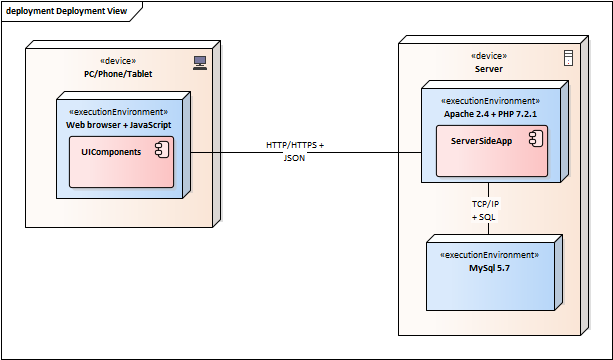
\includegraphics[width=\textwidth]{Deployment_view.png}
	\caption{Diagram nasazení}\label{deployment_view}
\end{figure}

\section{Uživatelská příručka}

\subsection{Tabulka}
	Tabulka\ref{tabulka} poskytuje možnosti pro manipulaci, procházení a vyhledávání tabulovaných dat. Jde o~následující funkce.
	\begin{description}
		\item[Výběr 1 řádky] je uskutečněn kliknutím na požadovanou řádku zároveň se stisknutím klávesy Ctrl. Opětovným kliknutím na tu samou řádku při zmáčkuté klávese Ctrl dojde ke zrušení výběru. Opakováním postupu lze vybrat více řádek.
		\item[Výběr více řádků] je docílen dvěma kroky. Nejprve označíme nebo odznačíme první krajní řádek výběru, tak jak bylo popsáno v~předchozím bodě. Poté klikneme zároveň se stlačenou klávesou Shift na druhou krajní řádku výběru. Tím dojde k~výběru všech řádek mezi krajními, včetně krajních.
		\item[Manipulace s~daty] -- úprava dat probíhá ve formulářích v~rámci modálního okna tabulky. Úpravy dat jsou potvrzené stisknutím tlačítka Save v~modálním. Zrušení změn pak tlačítkem Cancel. K~dispozici jsou tyto operace.
			\begin{description}
				\item[Nový záznam] -- stisknutím tlačítka \textbf{New} bude otevřen nevyplněný formulář pro zadání nového záznamu.
				\item[Editace záznamu] -- kliknutím na řádku s~požadovaným záznamem a následnou úpravou dat ve formuláři modálního okna.
				\item[Smazání záznamu(ů)] -- označením jednoho nebo více záznamů a následným stisknutím tlačítka \textbf{Delete}.
				\item[Hromadná editace] -- výběrem několika řádků a následným stisknutím tlačítka \textbf{Edit as one} dojde k~otevření formuláře pro zadání společných hodnot pro každý vybraný řádek.
			\end{description}
		\item[Filtrování] -- vložením hledaného výrazu do textového vstupu v~hlavičce tabulky a jeho potvrzení stisknutím klávesy Enter nebo kliknutím na tlačítko s~lupou. Výraz je vyhledán nad všemi sloupci.
		\item[Řazení] -- kliknutím na hlavičku sloupce budou záznamy seřazeny vzestupně dle hodnot v~daném sloupci. Opětovným stiskem se záznamy seřadí sestupně a třetím kliknutím bude řazení zrušeno.
		\item[Stránkování] -- pro procházení stránek se záznamy jsou určena tlačítka v~pravém dolním rohu tabulky. Kromě toho lze zvolit množství zobrazených záznamů na jedné stránce výběrem hodnoty v~sousedním select boxu.
		\item[Subtabulka] -- pro tabulky s~daty, které zahrnují i nějaká pomocná data, je možné zobrazit subtabulku kliknutím na malý trohúhelník na levém kraji řádky. Opětovným stisknutím tohoto trojúhelníku dojde ke skrytí subtabulky.
	\end{description}

\chapter{Testování}

\section{Testování}
	Testování aplikace primárně zajišťují jednotkové testy. Na úrovni jednotkových testů je také kontrolována správnost úprav dat, které aplikace zapisuje do databáze. Na aplikaci bylo také provedeno uživatelské testování použitelnosti, v~rámci kterého byly provedeny následující testovací scénáře.
	\begin{enumerate}
		\item Systém přijal objednávku na několik produktů. Zákazník v~objednávce požaduje odeslání objednávky, i když nebude kompletně skladem. Naplánujte expedici objednávky se zbožím, které je skladem. %Po přijetí tří objednávek expeditér připraví balíčky s požadovanými produkty. První objednávka je kompletně na skladě a bude vyřízena jedním balíčkem. Druhá objednávka je taktéž kompletně na skladě, ale expeditér produkty rozdělí do dvou balíčků. Třetí objednávka je pouze částečně na skladě, zákazník však požaduje odeslání objednávky, i přesto, že není kompletní. Expeditér tedy vytvoří balíček s produkty, které jsou na skladě.
		\item Po naplánování expedice objednávky jste zjistili, že rozložení produktů do dvou balíčků nebylo vhodné (zboží se do balíčků nevejde). Upravte expedici objednávky rozdělením produktů do tří balíčků.
		\item Do systému byly přijaty dvě samostatné objednávky od jednoho zákazníka. Zákazník u~druhé objednávky požaduje společné vyfakturování obou objednávek. Vytvořte fakturu na základě těchto dvou objednávek.
	\end{enumerate}



\begin{conclusion}
	%sem napište závěr Vaší práce
	%shrnutí míry uspěšnosti realizace cíle a jak jsme toho dosáhli
	%výhled do budoucna - možné rozšíření výsledku práce
	Cílem práce bylo navrhnout, implementovat a otestovat webový frontend informačního systému pro firmu MAHALUX s.r.o. na základě získaných funkčních a nefunkčních požadavků. Důraz byl kladen na použitelnost aplikace tak, aby napomáhala rychle a bezchybně zadávat data do databáze.
	
	U~vytvořeného prototypu se podařilo zajistit základní funkčnost. Aplikace zvládá obsluhu procesu vyřízení objednávky, včetně plánování expedice a fakturování objednávek. Je možné zobrazovat veškerá data z~databáze pomocí implementované tabulky, a dále je upravovat, mazat či přidávat nové záznamy. Pro vkládání a úpravy dat byly použity Nette formuláře. Zároveň se podařilo připravit API pro manipulaci se všemi tabulkami. Celá aplikace je postavena na návrhovém vzoru MVC, který je implementován spoluprací Nette prezenterů, Latté šablon a knihovny Doctrine 2. Nepodařilo se realizovat některé podpůrné prvky aplikace, jako je dynamické doplňování textu nebo vyplňování dat ze šablon. Do budoucna by měly být tyto funkce doplněny. 
	
	Aplikace je taktéž velice snadno rozšiřitelná a dobře konfigurovatelná. Díky tomu je možné provádět i poměrně velké změny v~databázovém modelu a v~návaznosti na to aplikaci jednoduše upravit. Kromě toho by bylo vhodné vytvořit proces Continous Deployment pro automatizované nasazování nových verzí systému včetně jeho testování.
\end{conclusion}

\bibliographystyle{csn690}
\bibliography{mybibliographyfile}

\appendix

\chapter{Seznam použitých zkratek}
% \printglossaries
\begin{description}
	\item[GUI] Graphical user interface
	\item[DDL] Data definition language
	\item[UML] Unified Modeling language
	\item[ORM] Object relation mapping
	\item[MVC] Model-view-controller
	\item[MVP] Model-view-presenter
	\item[DOM] Document Object Model
	\item[JSX] JavaScript Syntax eXtension
	\item[PDO] PHP Data Objects
	\item[API] Application interface
	\item[SQL] Structured Query Language
\end{description}


% % % % % % % % % % % % % % % % % % % % % % % % % % % % 
% % Tuto kapitolu z výsledné práce ODSTRAŇTE.
% % % % % % % % % % % % % % % % % % % % % % % % % % % % 
% 
% \chapter{Návod k~použití této šablony}
% 
% Tento dokument slouží jako základ pro napsání závěrečné práce na Fakultě informačních technologií ČVUT v~Praze.
% 
% \section{Výběr základu}
% 
% Vyberte si šablonu podle druhu práce (bakalářská, diplomová), jazyka (čeština, angličtina) a kódování (ASCII, \mbox{UTF-8}, \mbox{ISO-8859-2} neboli latin2 a nebo \mbox{Windows-1250}). 
% 
% V~české variantě naleznete šablony v~souborech pojmenovaných ve formátu práce\_kódování.tex. Typ může být:
% \begin{description}
% 	\item[BP] bakalářská práce,
% 	\item[DP] diplomová (magisterská) práce.
% \end{description}
% Kódování, ve kterém chcete psát, může být:
% \begin{description}
% 	\item[UTF-8] kódování Unicode,
% 	\item[ISO-8859-2] latin2,
% 	\item[Windows-1250] znaková sada 1250 Windows.
% \end{description}
% V~případě nejistoty ohledně kódování doporučujeme následující postup:
% \begin{enumerate}
% 	\item Otevřete šablony pro kódování UTF-8 v~editoru prostého textu, který chcete pro psaní práce použít -- pokud můžete texty s~diakritikou normálně přečíst, použijte tuto šablonu.
% 	\item V~opačném případě postupujte dále podle toho, jaký operační systém používáte:
% 	\begin{itemize}
% 		\item v~případě Windows použijte šablonu pro kódování \mbox{Windows-1250},
% 		\item jinak zkuste použít šablonu pro kódování \mbox{ISO-8859-2}.
% 	\end{itemize}
% \end{enumerate}
% 
% 
% V~anglické variantě jsou šablony pojmenované podle typu práce, možnosti jsou:
% \begin{description}
% 	\item[bachelors] bakalářská práce,
% 	\item[masters] diplomová (magisterská) práce.
% \end{description}
% 
% \section{Použití šablony}
% 
% Šablona je určena pro zpracování systémem \LaTeXe{}. Text je možné psát v~textovém editoru jako prostý text, lze však také využít specializovaný editor pro \LaTeX{}, např. Kile.
% 
% Pro získání tisknutelného výstupu z~takto vytvořeného souboru použijte příkaz \verb|pdflatex|, kterému předáte cestu k~souboru jako parametr. Vhodný editor pro \LaTeX{} toto udělá za Vás. \verb|pdfcslatex| ani \verb|cslatex| \emph{nebudou} s~těmito šablonami fungovat.
% 
% Více informací o~použití systému \LaTeX{} najdete např. v~\cite{wikilatex}.
% 
% \subsection{Typografie}
% 
% Při psaní dodržujte typografické konvence zvoleného jazyka. České \uv{uvozovky} zapisujte použitím příkazu \verb|\uv|, kterému v~parametru předáte text, jenž má být v~uvozovkách. Anglické otevírací uvozovky se v~\LaTeX{}u zadávají jako dva zpětné apostrofy, uzavírací uvozovky jako dva apostrofy. Často chybně uváděný symbol "{} (palce) nemá s~uvozovkami nic společného.
% 
% Dále je třeba zabránit zalomení řádky mezi některými slovy, v~češtině např. za jednopísmennými předložkami a spojkami (vyjma \uv{a}). To docílíte vložením pružné nezalomitelné mezery -- znakem \texttt{\textasciitilde}. V~tomto případě to není třeba dělat ručně, lze použít program \verb|vlna|.
% 
% Více o~typografii viz \cite{kobltypo}.
% 
% \subsection{Obrázky}
% 
% Pro umožnění vkládání obrázků je vhodné použít balíček \verb|graphicx|, samotné vložení se provede příkazem \verb|\includegraphics|. Takto je možné vkládat obrázky ve formátu PDF, PNG a JPEG jestliže používáte pdf\LaTeX{} nebo ve formátu EPS jestliže používáte \LaTeX{}. Doporučujeme preferovat vektorové obrázky před rastrovými (vyjma fotografií).
% 
% \subsubsection{Získání vhodného formátu}
% 
% Pro získání vektorových formátů PDF nebo EPS z~jiných lze použít některý z~vektorových grafických editorů. Pro převod rastrového obrázku na vektorový lze použít rasterizaci, kterou mnohé editory zvládají (např. Inkscape). Pro konverze lze použít též nástroje pro dávkové zpracování běžně dodávané s~\LaTeX{}em, např. \verb|epstopdf|.
% 
% \subsubsection{Plovoucí prostředí}
% 
% Příkazem \verb|\includegraphics| lze obrázky vkládat přímo, doporučujeme však použít plovoucí prostředí, konkrétně \verb|figure|. Například obrázek \ref{fig:float} byl vložen tímto způsobem. Vůbec přitom nevadí, když je obrázek umístěn jinde, než bylo původně zamýšleno -- je tomu tak hlavně kvůli dodržení typografických konvencí. Namísto vynucování konkrétní pozice obrázku doporučujeme používat odkazování z~textu (dvojice příkazů \verb|\label| a \verb|\ref|).
% 
% \begin{figure}\centering
% 	\includegraphics[width=0.5\textwidth, angle=30]{cvut-logo-bw}
% 	\caption[Příklad obrázku]{Ukázkový obrázek v~plovoucím prostředí}\label{fig:float}
% \end{figure}
% 
% \subsubsection{Verze obrázků}
% 
% % Gnuplot BW i barevně
% Může se hodit mít více verzí stejného obrázku, např. pro barevný či černobílý tisk a nebo pro prezentaci. S~pomocí některých nástrojů na generování grafiky je to snadné.
% 
% Máte-li například graf vytvořený v programu Gnuplot, můžete jeho černobílou variantu (viz obr. \ref{fig:gnuplot-bw}) vytvořit parametrem \verb|monochrome dashed| příkazu \verb|set term|. Barevnou variantu (viz obr. \ref{fig:gnuplot-col}) vhodnou na prezentace lze vytvořit parametrem \verb|colour solid|.
% 
% \begin{figure}\centering
% 	\includegraphics{gnuplot-bw}
% 	\caption{Černobílá varianta obrázku generovaného programem Gnuplot}\label{fig:gnuplot-bw}
% \end{figure}
% 
% \begin{figure}\centering
% 	\includegraphics{gnuplot-col}
% 	\caption{Barevná varianta obrázku generovaného programem Gnuplot}\label{fig:gnuplot-col}
% \end{figure}
% 
% 
% \subsection{Tabulky}
% 
% Tabulky lze zadávat různě, např. v~prostředí \verb|tabular|, avšak pro jejich vkládání platí to samé, co pro obrázky -- použijte plovoucí prostředí, v~tomto případě \verb|table|. Například tabulka \ref{tab:matematika} byla vložena tímto způsobem.
% 
% \begin{table}\centering
% 	\caption[Příklad tabulky]{Zadávání matematiky}\label{tab:matematika}
% 	\begin{tabular}{|l|l|c|c|}\hline
% 		Typ		& Prostředí		& \LaTeX{}ovská zkratka	& \TeX{}ovská zkratka	\tabularnewline \hline \hline
% 		Text		& \verb|math|		& \verb|\(...\)|	& \verb|$...$|		\tabularnewline \hline
% 		Displayed	& \verb|displaymath|	& \verb|\[...\]|	& \verb|$$...$$|	\tabularnewline \hline
% 	\end{tabular}
% \end{table}
% 
% % % % % % % % % % % % % % % % % % % % % % % % % % % % 

\chapter{Obsah přiloženého CD}

%upravte podle skutecnosti

\begin{figure}
	\dirtree{%
		.1 readme.txt\DTcomment{stručný popis obsahu CD}.
		.1 exe\DTcomment{adresář se spustitelnou formou implementace}.
		.1 src.
		.2 impl\DTcomment{zdrojové kódy implementace}.
		.2 thesis\DTcomment{zdrojová forma práce ve formátu \LaTeX{}}.
		.1 text\DTcomment{text práce}.
		.2 thesis.pdf\DTcomment{text práce ve formátu PDF}.
		.2 thesis.ps\DTcomment{text práce ve formátu PS}.
	}
\end{figure}

\end{document}
